The \DepthColorCam{} class represents a camera that provides fused depth-color images. It extends the 
\Camera{} abstract class, the base camera representation discussed in Section \ref{camera}. The 
implementation of the \DepthColorCam{} class, however, differs from that of the \ColorCam{} and 
\SwissRangerCam{} classes (see Sections \ref{colorcam} and \ref{swissrangercam}). The principal reason for 
the difference comes from the fact that instead of representing an actual sensor device, this class represents 
the merging of a depth camera with a color camera through the algorithmic process discussed in Section 
\ref{algorithm}.

In order to respond to this representation, the \DepthColorCam{} class instantiates a \SwissRangerCam{} 
object and a \ColorCam{} object. As discussed before, this means the acquired depth and color images can
either come directly from the cameras or be transferred through the network. Before obtaining the fused 
images, the depth-color camera needs to be calibrated using the \DepthColorCalibrationTool{}. This 
calibration tool provides the cameras' parameters needed by the \DepthColorFusion{} class to fuse the 
acquired depth and color images.

Table \ref{depthcolorcammethods} lists the methods of the \DepthColorCam{} class. The depth-color camera
object provides access to the fused image through the \texttt{get\-Fused\-Col\-or} and \texttt{get\-Depth}
methods. The first method returns the image buffer containing the color information of the fused image. The
second method returns the image buffer containing the depth information. The camera object also provides
access to the original color image (\texttt{get\-O\-rig\-i\-nal\-Col\-or}) and to the amplitude image associated 
with the depth measurements (\texttt{get\-Am\-pli\-tude}).

\begin{table}[ht]
\caption{Public methods in the \DepthColorCam{} class}
\begin{center}
\begin{tabular}{| l |}
	\hline 
	\multicolumn{1}{| c |}{\DepthColorCam{}} \\
	\multicolumn{1}{| c |}{{\small \texttt{extends} \Camera{}}} \\
	\hline \hline
	\texttt{getFusedColor} \\
	\texttt{getDepth} \\
	\texttt{getAmplitude} \\
	\texttt{getOriginalColor} \\
	\texttt{getDepthDisplay} \\
	\texttt{getAmplitudeDisplay} \\
	\texttt{getFusedColorView} \\
	\texttt{getDepthView} \\
	\texttt{getAmplitudeView} \\
	\texttt{getOriginalColorView} \\
	\texttt{getFusionTool} \\
	\texttt{getCalibrationTool} \\
	\texttt{getModulationFrequency} \\
	\texttt{setCameraParameters} \\
	\texttt{setupDepthColorFusion} \\
	\hline
\end{tabular}
\end{center}
\label{depthcolorcammethods}
\end{table}

Like the \SwissRangerCam{} class, the depth-color camera provides image buffers with the color
visualizations of the depth and amplitude images. These visualizations are obtained through the 
\texttt{get\-Depth\-Dis\-play} and \texttt{get\-Am\-pli\-tude\-Dis\-play} methods. Furthermore, all image streams
(fused color, depth, amplitude, and original color) are displayed in \RD{} using the \ImageView{} objects that 
are associated with each image buffer.

The rest of the methods are used to retrieve the modulation frequency on which the SwissRanger camera is
operating, to gain access to the \DepthColorCalibrationTool{} and \DepthColorFusion{} objects associated
with the depth-color camera, and to setup the depth-color fusion object after the camera has been calibrated. 

When capturing the image stream from the depth and color cameras, it is important to make sure that the
pair of acquired images belongs to the same point in time. Since the camera devices are different, the time
response of their capturing mechanisms is not identical. Furthermore, the transfer of the images from the 
cameras to the computer running \RD{} also accounts for the time difference between the 
images.\footnote{For example, the computer's processor speed might affect the image transfer time.}

To solve this synchronization problem, the depth-color camera uses the version of the \texttt{grab\-Im\-age} 
method in the \ColorCam{} and \SwissRangerCam{} objects that takes as input the desired timestamp of the 
image that will be grabbed (see Sections \ref{colorcam} and \ref{swissrangercam}). By using this method it is
possible to retrieve the two images closest in time while taking into account the timestamp offset. Table 
\ref{depthcolorgrabimage} describes the algorithm used by the \texttt{grab\-Im\-age} method in the 
depth-color camera to retrieve the depth and color images and produce the fused image.

\begin{table}[ht]
\caption[Algorithm for the \texttt{grabImage} method in \DepthColorCam{}]{Algorithm for the 
\texttt{grabImage} method in \DepthColorCam{}. The method returns \texttt{true} if the image  
was grabbed successfully and \texttt{false} otherwise.}
\begin{center}
\begin{tabular}{ l l }
\hline
\multicolumn{2}{l}{\texttt{GRAB\_IMAGE :}} \\
1 & \texttt{Grab image from color camera;} \\
2 & \texttt{{\bf If} the image is grabbed successfully} \\
3 & \hspace{0.6cm} \texttt{\bf Then:} \\
4 & \hspace{1.2cm} \texttt{Grab image from SwissRanger camera using as} \\
-  & \hspace{1.8cm} \texttt{input the timestamp of the color image;} \\
5 & \hspace{1.2cm} \texttt{{\bf If} the image is grabbed successfully} \\
6 & \hspace{1.8cm} \texttt{\bf Then:} \\
7 & \hspace{2.4cm} \texttt{Fuse the color and depth images;} \\
8 & \hspace{2.4cm} \texttt{Return true;} \\
9 & \hspace{1.8cm} \texttt{\bf Else:} \\
10 & \hspace{2.4cm} \texttt{Return false;} \\
11 & \hspace{0.6cm}\texttt{\bf Else:} \\
12 & \hspace{1.2cm} \texttt{Return false;} \\
\hline
\end{tabular}
\end{center}
\label{depthcolorgrabimage}
\end{table}

Another problem that arises with the depth-color camera involves the noisy nature of the SwissRanger
images. As mentioned in Section \ref{pointcorrespondences}, the noisy values for the $x$ and $y$ 
coordinates provided by the SwissRanger camera are discarded and recalculated using equations \eqref{X} 
and \eqref{Y}. The depth values, however, cannot be recalculated. The noise from the depth data produces 
a fused color image like the one shown in Figure \ref{noise}. In order to reduce this noise, some depth 
values are discarded based on depth and amplitude thresholds. Points that are too close, points that are too 
far, and points with small amplitude value are discarded. This produces areas with no depth and color 
information in the final fused depth-color image. 

\begin{figure}[t]
\center
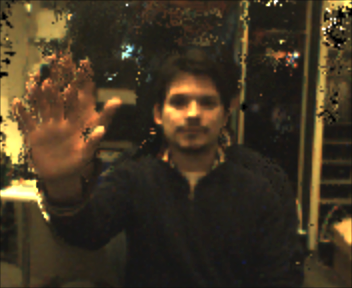
\includegraphics[scale = 0.5]{fusedcolornoise.png}
\caption{Fused color image without noise reduction}
\label{noise}
\end{figure}

Figure \ref{fusion} illustrates the result provided by the depth-color camera. It shows the original depth 
and color images, and next to them the fused color image. The black pixels in the depth and fused color
images indicate the points that were discarded due to data noise. It is worth noting that by thresholding the 
depth image it is possible to segment the object of interest from the background. 

\begin{figure}[t]
\center
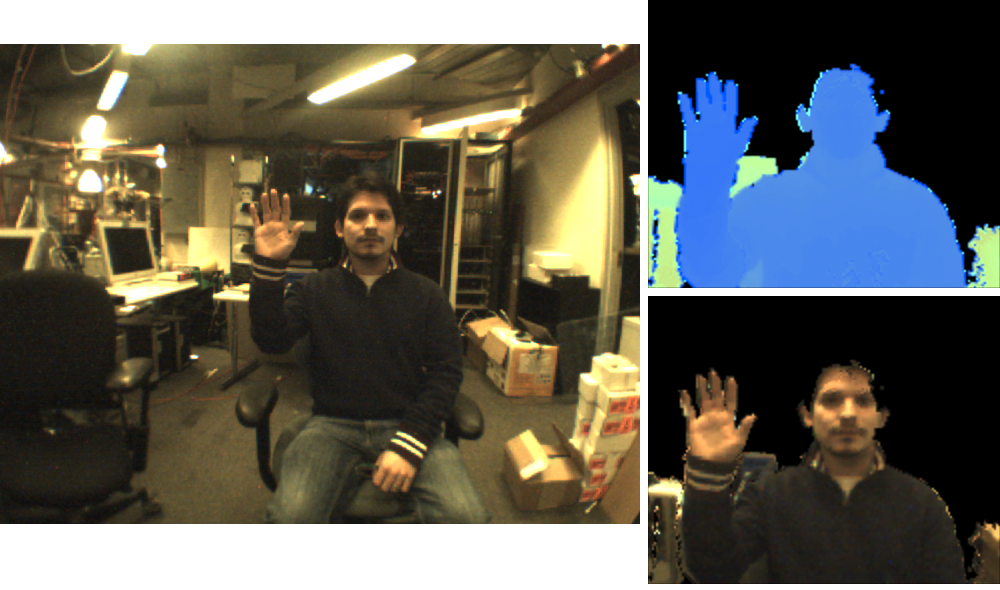
\includegraphics[width = 15cm]{fusion.png}
\caption[\DepthColorCam{}'s images]{\DepthColorCam{}'s images: the original color image (left), the 
depth image (upper right) and the fused color image (bottom right).}
\label{fusion}
\end{figure}


